\section{Machine Learning Recap}
\textbf{Artificial Intelligence} (AI) is the discipline that aims to create machines that mimic human intelligence.
\textbf{Machine Learning} (ML) is a subset of AI that enables machines to learn from experience (i.e., data) to improve their performance on a specific task.
\textbf{Deep Learning} is in turn a subfield of ML that focuses on \textbf{Artificial Neural Networks} (ANNs); the term `deep' refers to the use of multiple layers,
which allows the network to learn complex representations of data with multiple levels of abstraction.

Machine Learning was born in contrast to the programming paradigm, which is based on the idea of writing explicit rules to solve a problem.
\begin{figure}[H]
    \centering
    \scalebox{0.8}{
        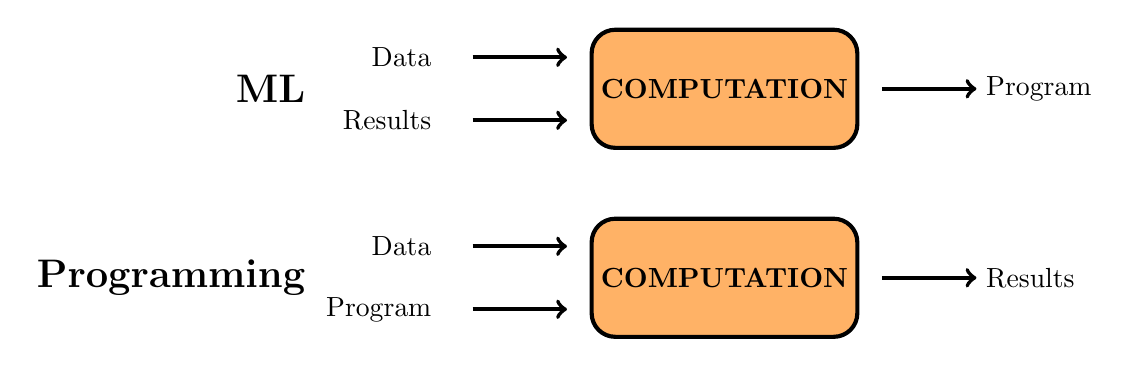
\begin{tikzpicture}[scale=0.8]
  % Styling
  \tikzset{
    box/.style={
      rectangle,
      rounded corners=0.3cm,
      minimum width=3cm,
      minimum height=1.5cm,
      fill=orange!60,
      draw=black,
      line width=1.5pt,
      font=\bfseries
    },
    arrow/.style={
      ->,
      line width=1.5pt,
      black
    },
    label/.style={
      font=\normalsize,
      black
    },
    bigLabel/.style={
      font=\Large\bfseries,
      black
    }
  }
  
  % ===== Machine Learning =====
  \node[bigLabel, left] at (-3, 3) {ML};
  % Input labels
  \node[label, left] at (-1, 3.5) {Data};
  \node[label, left] at (-1, 2.5) {Results};
  
  % Arrows from inputs
  \draw[arrow] (-0.5, 3.5) -- (1, 3.5);
  \draw[arrow] (-0.5, 2.5) -- (1, 2.5);
  
  % Main computation box
  \node[box] (comp1) at (3.5, 3) {COMPUTATION};
  
  % Arrow to output
  \draw[arrow] (6, 3) -- (7.5, 3);
  
  % Output label
  \node[label, right] at (7.5, 3) {Program};
  
  % ===== Programming Approach =====
  \node[bigLabel, left] at (-3, 0) {Programming};
  % Input labels
  \node[label, left] at (-1, 0.5) {Data};
  \node[label, left] at (-1, -0.5) {Program};
  
  % Arrows from inputs
  \draw[arrow] (-0.5, 0.5) -- (1, 0.5);
  \draw[arrow] (-0.5, -0.5) -- (1, -0.5);
  
  % Main computation box
  \node[box] (comp2) at (3.5, 0) {COMPUTATION};
  
  % Arrow to output
  \draw[arrow] (6, 0) -- (7.5, 0);
  
  % Output label
  \node[label, right] at (7.5, 0) {Results};
  
\end{tikzpicture}

    }
    \caption{Programming paradigm vs Machine Learning paradigm.}
    \label{fig:programming_paradigm}
\end{figure}
In the Machine Learning paradigm, we are instead given the data, along with the results, and we try to learn the \textbf{model}. The learned model
(e.g. splits in a decision tree, linear function for SVMs) represents the solution to the problem, and it can be used to make predictions on new data.

\subsection{Why do we need Machine Learning}
The main reason why we need Machine Learning can be summarized in the following points:
\begin{itemize}
    \item \textbf{Complexity of the problem}: For many tasks, we have no human expertise to write explicit rules;
    \item \textbf{Personalized solutions}: For many tasks, we need to learn personalized solutions for each user, which is not feasible with the programming paradigm;
    \item \textbf{Huge amount of data}: Working with huge amount of data is not feasible, as it would require writing down explicit rules for each possible combination of inputs.
\end{itemize}

\subsection{Machine Learning - Another definition}
\definition{Machine Learning}{
    A computer program is said to learn from experience $E$ with respect to some class of tasks $T$
    and performance measure $P$, if its performance at tasks in $T$, as measured by $P$, improves with
    experience $E$.
}
This definition is more formal and precise than the previous one, and it highlights the importance of the three components: experience, task, and performance measure.
Each machine learning algorithm can be characterized by these three components. For example, taking in consideration a spam email filter, we can define:
\begin{itemize}
    \item $T$: Categorizing emails as spam or not spam;
    \item $P$: Accuracy of the classification. Other metrics may be more appropriate;
    \item $E$: Database of emails labeled as spam or not spam by human experts.
\end{itemize}

\subsection{Types of learning}
We can identify three main types of learning:
\begin{itemize}
    \item \textbf{Supervised learning}: We are given a training set of input-output pairs, and we want to learn a function that maps inputs to outputs.
    \item \textbf{Unsupervised learning}: We are given a training set of inputs, and we want to learn a function that captures the underlying structure of the data.
    \item \textbf{Reinforcement learning}: We are given an environment, and we want to learn a policy that maximizes the cumulative reward.
\end{itemize}

\subsubsection{Supervised Learning}
Supervised learning can be further divided into subcategories, such as:
\begin{itemize}
    \item \textbf{Classification}: The output is a discrete label. More formally, given a training set $\mathcal{D} = \{(\mathbf{x}_1, y_1), \dots, (\mathbf{x}_n, y_n)\}$ we can define it as:
    \begin{equation}
        f: \mathcal{X} \rightarrow \{1,\dots,k\}
    \end{equation}
    where $\mathcal{X}$ is the input space, and $\{1,\dots,k\}$ is the set of possible labels.
    
    Based on the number of classes, we can further divide classification into \textbf{binary classification} and \textbf{multi-class classification}.
    
    \item \textbf{Regression}: The output is a continuous value. More formally, given a training set $\mathcal{D} = \{(\mathbf{x}_1, y_1), \dots, (\mathbf{x}_n, y_n)\}$ we can define it as:
    \begin{equation}
        f: \mathcal{X} \rightarrow \mathbb{R}
    \end{equation}
    
    \item \textbf{Structured output}: \textbf{supervised learning} doesn't necessarily require a \textbf{vector} as input, and a \textbf{scalar} as output.
    We can have more complex input and output structures, such as images, graphs, or sequences.
    In all cases the output  is a structured object, with relationships between its components.
    Some practical example of \textbf{structured input regression} problems are:
    
    \begin{itemize}
        \item \textbf{Semantic segmentation}: Given an image of input size $M \times N \times 3$, we
        want to predict a mask of size $M \times N$, where each pixel is labeled with a class.
        The original solution to this kind of problem was to use \textbf{feature engineering} to extract features from neighborhoods of pixels. After that,
        SVMs were used to make predictions based on the extracted features. \textbf{Neural Networks} show their real power in this kind of problems,
        as they are able to learn features directly from the data, without any human intervention.
        
        \item \textbf{Machine translation}: given a sentence (sequence of words) in a source language, we want to translate it
        to a target language. This is even more complex than the previous example, as not only the output is related to its adjacent components,
        but also grammatical and semantic relationships between words need to be captured.
    \end{itemize}
\end{itemize}

\begin{comment}
    Add image for Deep Clustering and Deep Generative Models
\end{comment}
\subsubsection{Unsupervised Learning}
In unsupervised learning, we are given a training set of inputs, without any corresponding output labels, 
and we want to learn the underlying structure of the data. Some examples of unsupervised learning tasks are:
\begin{itemize}
    \item \textbf{Clustering}: grouping similar data points together;
    
    \item \textbf{Deep clustering}: a technique that combines deep learning with classical clustering algorithms, such as k-means,
    to learn better representations of the data and improve clustering performance.
    It is based on the idea of using a deep neural network to learn a low-dimensional representation of the data. This
    is then used as input to a clustering algorithm, producing a set of \textbf{pseudo-labels} that are used to train the neural network
    using backpropagation. This process is repeated iteratively until convergence;
    \begin{figure}[H]
        \centering
        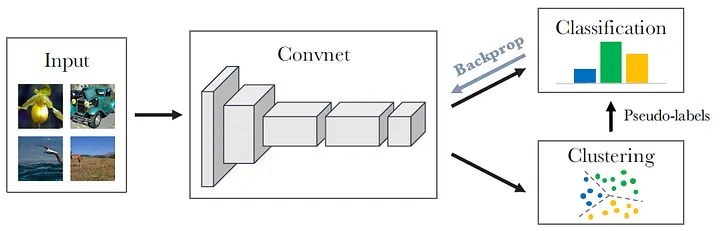
\includegraphics[width=\textwidth]{chapters/01-ml-recap/media/deep_clustering.png}
        \caption{Deep clustering.}
    \end{figure}
    \item \textbf{Generative Models}: models learn the underlying distribution of the data,
    and can be used to generate new data points, similar to the ones in the training set.
    Also in this case, we can have \textbf{deep generative models}. They try to map exaples extracted from a simple distribution $Z$ to a more complex distribution $g_{\theta}(Z)$,
    which is similar to the distribution of $X$.
    \begin{figure}[H]
        \centering
        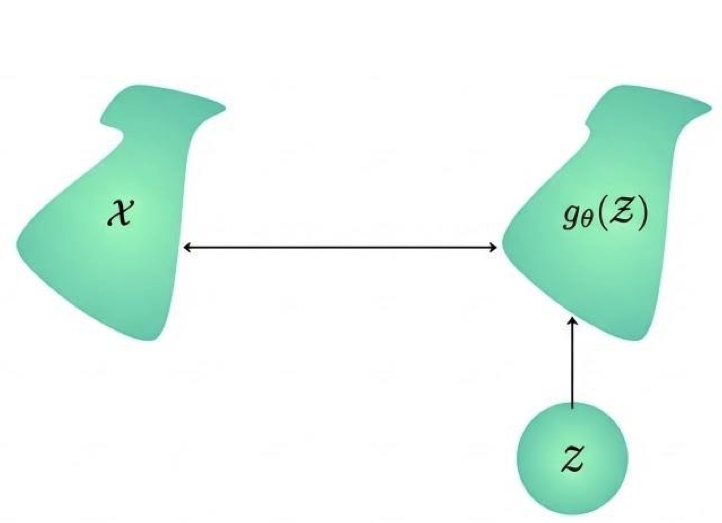
\includegraphics[width=0.5\textwidth]{chapters/01-ml-recap/media/deep_generative_models.png}
        \caption{Deep generative models.}
    \end{figure}

    \item \textbf{Dimensionality reduction}: try to map data to a lower-dimensional space in which
    visualization and interpretation are easier. This is often used as a preprocessing step for other machine learning algorithms.

    \item \textbf{Autoencoders}: a type of encoder-decoder architecture, where:
    \begin{itemize}
        \item The \textbf{encoder} maps the input data to a \textbf{latent space} of lower dimensionality;
        \item The \textbf{decoder} maps the latent representation back to the original input.
    \end{itemize}
    The two components are trained together to minimize the reconstruction error, which is the difference between the original input and the reconstructed output.
    Once trained, the encoder can be used alone to obtain lower-dimensional representations of the data.
\end{itemize}

\subsubsection{Reinforcement Learning}
In Reinforcement Learning, an \textbf{agent} learn to interact with an \textbf{environment} in order to maximize a cumulative reward.
We are not given any data, but rather the agent learns from its own experience, by exploring the environment and receiving feedback in the form of rewards.

In \textbf{deep reinforcement learning} the agent uses a deep neural network to learn a policy that maps states of the environment to actions. 
This allows the agent to learn complex behaviors and solve tasks that are difficult to solve with traditional reinforcement learning algorithms.

\subsection{Designing a Learning System}
To design a learning system, it's important to consider the following steps:
\begin{enumerate}
    \item \textbf{Choose the training experience $E$}: This is the data that will be used to train the model.
    It should be representative of the problem we want to solve, and it should be of good quality;
    \item \textbf{Choose the model}: This is the function that we want to learn from the data.
    It heavily depends on the task we want to solve,
    \item \textbf{Choose how to represent the model}: the form of the model, what kind of function we allow. For example, we can have:
    \begin{itemize}
        \item \textbf{Instance-based functions}: predictions are made based on the similarity between the input and the training examples. For example, k-nearest neighbors;
        \item \textbf{Numerical functions}: predictions are made based on a mathematical function that maps inputs to outputs. For example, Neural Networks, SVMs;
        \item \textbf{Probabilistic functions}: predictions are made based on a probability distribution over the possible outputs. For example, Naive Bayes;
        \item \textbf{Symbolic functions}: predictions are made based on a set of rules that are learned from the data. For example, decision trees.
    \end{itemize}
    \item \textbf{Choose the learning algorithm}: This is the algorithm that will be used to learn the model from the data.
    For example, for SVMs we can decide between different optimization algorithms, such as stochastic gradient descent or
    quadratic optimization.

    The success of the machine learning system also depends on the search and optimization algorithm used to find the best model.
    \item \textbf{Choose the performance measure $P$}: This is the metric that will be used to evaluate the performance of the model.
    Different tasks require different performance measures and it's not always a trivial choice. Ideally we would like to choose a performance measure that is closely related
    to the loss function used to train the model.
\end{enumerate}

\subsection{Assumptions in Machine Learning}
When developing a machine learning model, we usually assume that we are given a training set of examples that are \textbf{observed}
and we want to learn a model that can make predictions on new, unseen examples, the \textbf{test set}.

The challenge is that the algorithm has to learn a model that performs well on new examples. This ability is known as \textbf{generalization}.

\subsubsection{Empirical risk minimization}
Classical optimization algorithms are different from machine learning algorithms. 
In classical optimization, the only goal is to find the best solution to a problem, reducing the \textbf{training error} as much as possible.
In machine learning instead, we want to minimize the \textbf{test error}, which is the error on new, unseen examples. 
This is a much harder problem, as we don't have direct access to the test set during training.

To tackle this problem, we assume that both training and test examples are drawn from the same
distribution. This is known as the \textbf{independent and identically distributed} (i.i.d.) assumption, and it allows us to use the 
training set to learn a model that generalizes well to the test set.

If the training set is representative of the underlying unknown distribution, then the \textbf{empirical loss} (the average loss on the training set)
is a good estimate of the \textbf{expected loss} (the average loss on the test set). 
This is the principle of \textbf{empirical risk minimization}.

\subsubsection{Assumption violations}
If the training set is not representative of the underlying distribution or if the i.i.d. assumption is violated,
then the model may not generalize well to the test set, and we may end up with a model that performs well on the training set but poorly on the test set. This is known as \textbf{overfitting}.

\subsubsection{Underfitting}
If the model is too simple, it may perform poorly on both the training and test set. This is known as \textbf{underfitting}.
To avoid underfitting, we need to choose a more complex model, or to use a more powerful learning algorithm.

\subsubsection{Overfitting}
If the model is too complex, it may perform well on the training set but poorly on the test set. 
When the gap between the two errors is large, it means that the model has learned to fit the noise in the training data, rather than the underlying distribution.
This is known as \textbf{overfitting}.

To avoid overfitting, we can use techniques such as:
\begin{itemize}
    \item \textbf{Simpler models}: choosing a simpler model with fewer parameters, which is less likely to overfit the training data;
    \item \textbf{Regularization}: any modification made to a learning algorithm that is intended to reduce the generalization error, but not the training error. Usually,
    this is done by adding a penalty term to the loss function, which is proportional to the complexity of the model (e.g., adding a term that penalizes large weights in a neural network).
\end{itemize}

\subsection{How to choose the algorithm}
To choose the right algorithm for a given problem, we need to consider the following factors:
\begin{itemize}
    \item \textbf{Size of the training set}: Some algorithms perform better with small training sets, while others require large training sets to perform well;
    \item \textbf{Address problem difficulty}: are data linearly separable? Is the problem a regression or a classification problem? Is the output structured?
    \item \textbf{Prior knowledge}: if prior knowledge about the problem is available, it can be encoded in the model, which can improve performance;
    \item \textbf{Computational requirements}: do we have any requirements on the computational resources available for training and inference?
    \item \textbf{Online vs batch learning}: based on the kind of data we have, we may need to choose different algorithms. For example, for streaming data,
    Neural Network aren't the best choice;
    \item \textbf{Interpretability}: do we need to understand how the model makes predictions?
\end{itemize}